\documentclass[../dissertation.tex]{subfiles}
\begin{document}

\chapter{Design}

\section{Scoping}

The goal of the project will be, primarily, to make an effective web wrapper for the Tulip Python API. This would take requests from a client, that would include a file ID (for a file stored locally or elsewhere), and any other parameters such as how much data to return (depending on machine power / network connection) or type of reducing to do.

There will also be, at least, a basic interface that will allow for interactions to be made with the web endpoint, and the requirement that the system has benefits over not using the web endpoint (i.e. sending the file directly from the storage to the interface).

Ideally, the web endpoint will be made flexible enough to allow for a large proportion of the useful parts of the Tulip API to be made available, allowing for other developers to make their own client to interface with it. On top of that, ideally the JavaScript client would not be hardcoded but be a library that the interface would use in order to communicate with the web endpoint. This would allow for other developers to use make their own interface to use with the JavaScript Client and Web Endpoint.

Some features that will be included if time allows are the ability for the user to ask for an image as opposed to a network  of nodes to be returned, if, for example, the machine they are using is underpowered or has a bad network connection, along with the ability to have the web wrapper communicate with an external data host. This would be useful if the users machines have little file storage.

Finally, it would be nice to have a fully-fledged interface to allow for a pleasant and easy user experience with all options available to the user. However, given time constraints, this may not be possible.

\section{Requirements}

At this point, the MoSCoW method was used to create a set of requirements for the system, with differing priorities.

Must Have:
\begin{itemize}
    \item A web endpoint that calls the Tulip Python API
	\item To be able to deal with large data (that is too large to just send of the network and be visualised be the client without manipulation)
	\item A basic demo interface
	\item To have render-able data returned from the endpoint
\end{itemize}

Should Have:
\begin{itemize}
    \item A neat JavaScript Client, with neat meaning a well-documented list of functions that the client can call that then make calls to the web end-point
	\item A flexible web endpoint, with flexible meaning covers as many relevant API calls as possible, and making sure that as few of the parameters for the API calls are hard-coded. This has the benefit of both:
	\begin{itemize}
	    \item Making the system more useful for a larger number of clients
        \item Letting clients make more than just JavaScript clients, so if they want to make a C\# or Java app that wouldn't be a problem
	\end{itemize}
\end{itemize}
	
Could Have:
\begin{itemize}
    \item The ability to ask for an image to be returned if client is low power
	\item The ability to interface with an external data host (like S3) (could look into using Hadoop)
\end{itemize}
	
Probably Won't Have:
\begin{itemize}
    \item A fully fledged and pretty interface
\end{itemize}
	

\section{Design Decisions}

Justification for including or not including the following features:

\subsection{Web Endpoint}

This is the most core part of the project, creating a web wrapper for the Tulip Python API. The justification for making this is to allow low spec clients (low processing power / RAM / storage) to visualise data quickly. Currently alternatives include using spreadsheet software which takes a long time and isn't very meaningful, or using graphing software, but that requires installing the software locally. Making a web wrapper for Tulip would allow a client to log in to a system and visualise a potentially massive network quickly and easily due to all of the processing of the graph done on a powerful server. Also, assuming that the software will be dealing with a massive data (a user could have access to TBs of data) then it is not feasible that any client could store that locally.

\subsection{A Basic Interface}

Although the interface will probably not be very complicated, it is important to have some form of interface in order to demo the product and show the whole system working

Better than without - It is necessary that in the vast majority of (or all) cases that the system works better using the web wrapper than just passing the nodes directly to the client. There should be an large increase in performance as the amount of data gets higher.

\subsection{Making the web wrapper flexible}
This is not essential for allowing the creation of the application, but if I am to make a program for this project, it would be highly preferable to create an API that other developers can hook into and use easily. This involves making all the API calls as open as possible and covering as much as possible, and also making sure it is well documented.

\subsection{JS Library}
In a similar vein, as opposed to just making an interface that has all of the JavaScript calling the web endpoint as part of it, it would be preferable to make a JS library that would interface with the web endpoint, and then the client would call the JS library. This would make it far easier for developers to develop their own client using the library and the web endpoint, which could be hooked into their own data source easily.

\subsection{Return an image}
As opposed to return a blob of data including nodes and edges, and ways to visualise them, it would be nice to allow for the user to select an option to just return an image of the graph. This would allow for the system to work on very low power machines or machines with a bad network connection.

\subsection{Fully fledged interface}
This would make the product look more finished off and neat, but is not required in order for the project to be complete as the developers for users of the system would be expected to make their own interface.

\section{Technical Infrastructure}

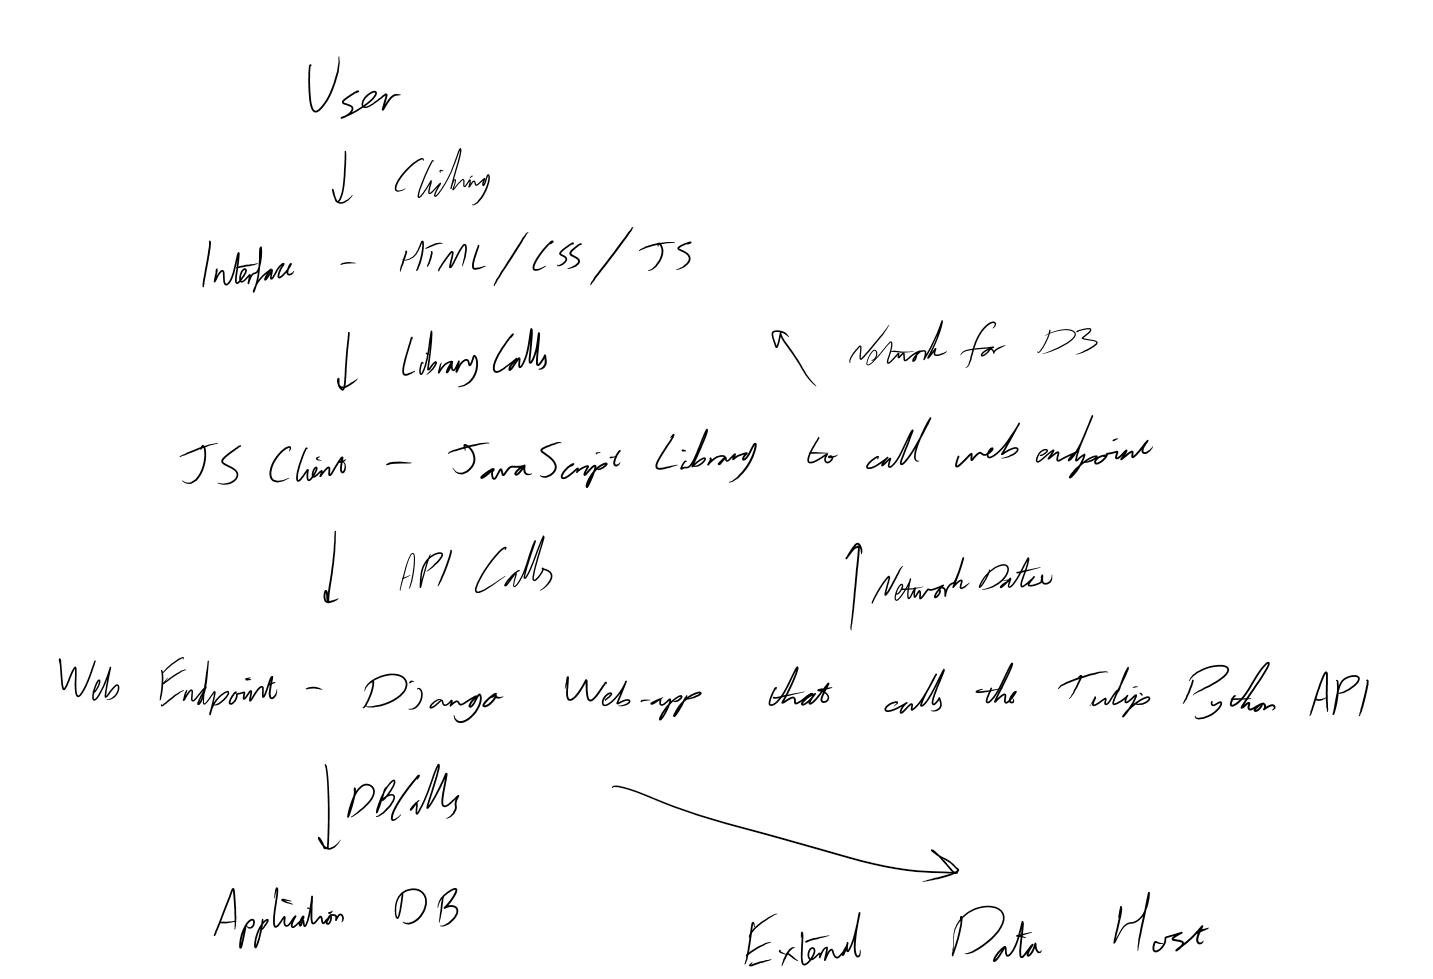
\includegraphics[width=17cm]{5/tech_infra}

\subsection{Sample Data Flow}

{\centering
Click Load Network
\\$\downarrow$\\
Name Network
\\$\downarrow$\\
Network details saved in system and network saved in external data host
\\$\downarrow$\\ 
Click Open Network and select network to open
\\$\downarrow$\\
Request sent to back end for network
\\$\downarrow$\\
Database queried for network and location on external data host found
\\$\downarrow$\\
External Data Host sends network data to back end
\\$\downarrow$\\ 
Back end uses Tulip Python API to shrink the data and make it easier to send over a network
\\$\downarrow$\\
New smaller network send over network to JS Client
\\$\downarrow$\\
D3.js renders the network which is interactive\\
}

\end{document}